\begin{frame}
	\frametitle{caso di studio: Reid [2011]}
	\framesubtitle{rete transazioni $\mathcal{T}$}

	\begin{figure}[H]
	 	\begin{center}
			 \begin{tabular}{c @{\hspace{1em}} c}
				 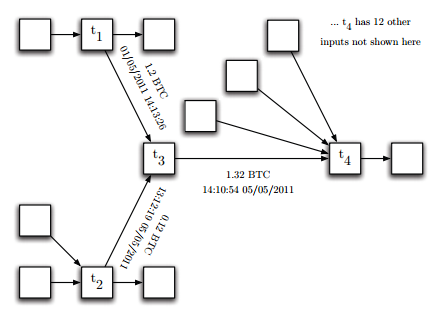
\includegraphics[height=6 cm]{images/anon_1.png}
			 \end{tabular}
		 \end{center}
 	\end{figure}

\end{frame}

\begin{frame}
	\frametitle{caso di studio: Reid [2011]}
	\framesubtitle{rete utenti imperfetta $\tilde{\mathcal{U}}$ }

	\begin{figure}[H]
	 	\begin{center}
			 \begin{tabular}{c @{\hspace{1em}} c}
				 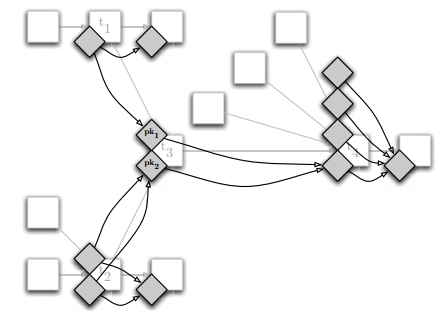
\includegraphics[height=6 cm]{images/anon_2.png}
			 \end{tabular}
		 \end{center}
 	\end{figure}
 
\end{frame}

\begin{frame}
	\frametitle{caso di studio: Reid [2011]}
	\framesubtitle{rete utenti $\mathcal{U}$, rete ancella $\mathcal{A}$}
	
	\begin{figure}[H]
	 	\begin{center}
			 \begin{tabular}{c @{\hspace{1em}} c}
				 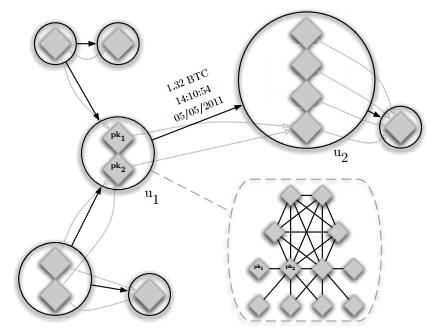
\includegraphics[height=6 cm]{images/anon_3.png}
			 \end{tabular}
		 \end{center}
 	\end{figure}

\end{frame}

\begin{frame}
	\frametitle{caso di studio: Reid [2011]}
	\framesubtitle{integrazione con informazioni esterne}
	
	\begin{itemize}
		\item dimensione $\propto |\{K_{PB}\}|$ utente = \# transazioni
		\item colore $\propto$ \bitcoinA \;scambiati
	\end{itemize} 
	
	\begin{figure}[H]
	 	\begin{center}
			 \begin{tabular}{c @{\hspace{1em}} c}
				 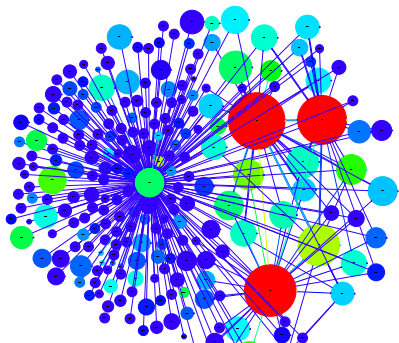
\includegraphics[height=6 cm]{images/anon_4.png}
			 \end{tabular}
		 \end{center}
 	\end{figure}

\end{frame}